\chapter{Algorithm to obtain Faithful Clustering}
In this chapter we have a closer look at the algorithms we designed and how they work. We provide an explanation, accompanied with an example and pseudo-code.
In \cref{sec:ConcretizingSingletons} we explain, the concretization of a clustered argument. Next, in \cref{sec:ComputationOfConcretizerList} we explain how the concretizer list (a list of clustered arguments which are mutated to singletons) is computed. The approach to compute faithful clustered AFs is described in \cref{sec:AlgorithmicApproachToComputeFaifthulClusterings}. And finally we state the heuristics and refinements in \cref{sec:HeuristicsAndRefinements}.

\textit{TODO: Update when adding sections}

\section{Concretizing Singletons}
\label{sec:ConcretizingSingletons}
When operating on clustered AFs, a crucial mutation is to extract clustered arguments from a cluster and transform it to a singleton. This is called concretizing. When clustering singletons, the cluster inherits the attacks of the argument, concretizing is the inverse operation. This means, that it needs to revert the changes done by the clustering.
Concretizing a list of arguments is done iteratively by duplicating the abstract AF $\hat{F}$ to create a new AF $\hat{F}'$ and transforming it. The transformation is guided by five steps considering the unchanged abstract AF $\hat{F}$ and the concrete AF $F$. To improve the understanding of each step, we accompany the explanation with the example depicted in \cref{example:concretizationOfArguments}, where we concretize the arguments $a$ and $b$.

\vspace{0.3cm}

\vspace{0.3cm}
\begin{figure}[h]
    \centering
    \begin{subfigure}[b]{0.475\textwidth}
        \centering
        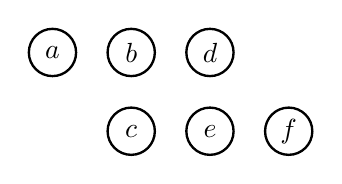
\begin{tikzpicture}
            % Singletons
                \def \ax{0}   \def \ay{0}
                \def \bx{1}   \def \by{0}
                \def \cx{1}   \def \cy{-1}
                \def \dx{2}   \def \dy{0}
                \def \ex{2}   \def \ey{-1}
                \def \fx{3}   \def \fy{-1}

                \draw[line width=0.3mm] (\ax, \ay) circle (0.3) node[anchor=center]{$a$};
                \draw[line width=0.3mm] (\bx, \by) circle (0.3) node[anchor=center]{$b$};
                \draw[line width=0.3mm] (\cx, \cy) circle (0.3) node[anchor=center]{$c$};
                \draw[line width=0.3mm] (\dx, \dy) circle (0.3) node[anchor=center]{$d$};
                \draw[line width=0.3mm] (\ex, \ey) circle (0.3) node[anchor=center]{$e$};
                \draw[line width=0.3mm] (\fx, \fy) circle (0.3) node[anchor=center]{$f$};
                % Attacks
                \DrawAttackHorizontal{L}{\bx}{\by}{\ax}{\ay}
                \DrawAttackHorizontal{L}{\dx}{\dy}{\bx}{\by}

                \DrawAttackVertical{D}{\bx}{\by}{\cx}{\cy}
                \DrawAttackVertical{U}{\ex}{\ey}{\dx}{\dy}

                \DrawAttackDiagonal{NRL}{\cx}{\cy}{\ax}{\ay}
        \end{tikzpicture}
        \caption{Concrete AF $F$}
        \label{fig:concrete_af}
    \end{subfigure}%
    \hfill
    \begin{subfigure}[b]{0.475\textwidth}
        \centering
        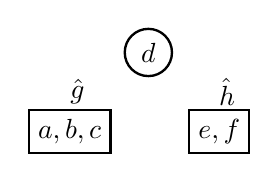
\begin{tikzpicture}
            % Singletons
            \def \dx{1}   \def \dy{0}
            \def \gx{0}   \def \gy{-1}
            \def \hx{1.9}   \def \hy{-1}

            \draw[line width=0.3mm] (\dx, \dy) circle (0.3) node[anchor=center]{$d$};
            % Cluster

            \node[rectangle, draw, line width=0.3mm] at (\gx, \gy) {$a,b,c$};
            \node at (\gx + 0.1, \gy+0.5) {$\hat{g}$};

            \node[rectangle, draw, line width=0.3mm] at (\hx, \hy) {$e,f$};
            \node at (\hx + 0.1, \hy+0.5) {$\hat{h}$};

            % Attacks
            \DrawAttackDiagonal{PRL}{\dx}{\dy}{\gx+0.1}{\gy+0.1}
            \DrawAttackDiagonal{NRL}{\hx}{\hy+0.1}{\dx}{\dy}
            \DrawSelfAttackLeftTopCluster{\gx-0.45}{\gy+0.3}
        \end{tikzpicture}
        \caption{Abstract AF $\hat{F}$}
        \label{fig:abstract_af}
    \end{subfigure}
    \caption{Concrete and abstract AF}
    \label{example:concretizationOfArguments}
\end{figure}

\paragraph{Step 1:} Each argument needing concretization is first removed from the parent cluster and added as a singleton in $\hat{F}'$.
If an argument is not part of a cluster, we ignore it.
We do not consider attacks in this step since they depend on the concrete- and abstract AFs. The resulting AF is depicted in \cref{example:algorithmConcretizeSingletonsStep1} and the pseudo-code in \cref{alg:concretizingSingletonsStep1}.


\vspace{0.3cm}
\begin{figure}[h]
    \centering
    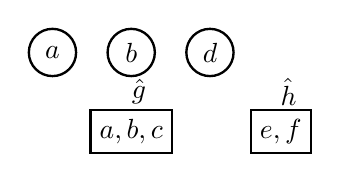
\begin{tikzpicture}
        % Singletons
        \def \ax{0}   \def \ay{0}
        \def \bx{1}   \def \by{0}
        \def \dx{2}   \def \dy{0}
        \def \gx{1}   \def \gy{-1}
        \def \hx{2.9}   \def \hy{-1}

        \draw[line width=0.3mm] (\ax, \ay) circle (0.3) node[anchor=center]{$a$};
        \draw[line width=0.3mm] (\bx, \by) circle (0.3) node[anchor=center]{$b$};
        \draw[line width=0.3mm] (\dx, \dy) circle (0.3) node[anchor=center]{$d$};
        % Cluster

        \node[rectangle, draw, line width=0.3mm] at (\gx, \gy) {$a,b,c$};
        \node at (\gx + 0.1, \gy + 0.5) {$\hat{g}$};

        \node[rectangle, draw, line width=0.3mm] at (\hx, \hy) {$e,f$};
        \node at (\hx + 0.1, \hy + 0.5) {$\hat{h}$};

        % Attacks
        \DrawAttackDiagonal{PRL}{\dx}{\dy}{\gx+0.1}{\gy+0.1}
        \DrawAttackDiagonal{NRL}{\hx}{\hy+0.1}{\dx}{\dy}
        \DrawSelfAttackLeftTopCluster{\gx-0.45}{\gy+0.3}

    \end{tikzpicture}
    \caption{Concretized AF $\hat{F}'$ after Step 1}
    \label{example:algorithmConcretizeSingletonsStep1}
\end{figure}
\vspace{-0.2cm}


\begin{algorithm}[H]
    \caption{Concretizing Singletons Pseudocode Step 1}\label{alg:concretizingSingletonsStep1}
    \begin{algorithmic}[1]
        \Require $A: AF(a_1, r_1)$ \Comment{Abstract Clustered AF}
        \Require $e: list(Arguments)$ \Comment{Concretizer List}
        \State $N$ $\gets$ $A$ \Comment{$N$ = Concretized Cluster}
        \For{$a_i$ in $e$}
            \For{$c_i$ in $A.clusters$}
                \If{$a_i$ in $c_i$}
                    \State $c_i.remove(a_i)$
                \EndIf
                \EndFor
            \State $N.addSingleton(a_i)$
        \EndFor
    \end{algorithmic}
\end{algorithm}




\paragraph{Step 2:} We add the new attacks from all concretized arguments to the remaining clusters and vice versa. We must do this after removing the arguments from the clusters because if an argument $a$ attacks argument $b$ in the concrete AF $F$, and $b$ is part of the cluster $\hat{g}$ in the abstract AF $\hat{F}$, by concretizing $b$, the attack $(a,\hat{g})$ would not be present anymore. The resulting AF $\hat{F}'$ is depicted in \cref{example:algorithmConcretizeSingletonsStep2} and the pseudo-code in \cref{alg:concretizingSingletonsStep2}


\vspace{0.3cm}
\begin{figure}[h]
    \centering
    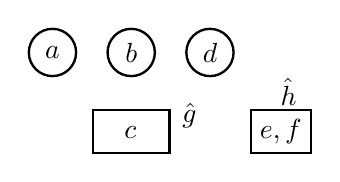
\begin{tikzpicture}
        % Singletons
        \def \ax{0}   \def \ay{0}
        \def \bx{1}   \def \by{0}
        \def \dx{2}   \def \dy{0}
        \def \gx{1}   \def \gy{-1}
        \def \hx{2.9}   \def \hy{-1}

        \draw[line width=0.3mm] (\ax, \ay) circle (0.3) node[anchor=center]{$a$};
        \draw[line width=0.3mm] (\bx, \by) circle (0.3) node[anchor=center]{$b$};
        \draw[line width=0.3mm] (\dx, \dy) circle (0.3) node[anchor=center]{$d$};
        % Cluster

        \node[rectangle, draw, line width=0.3mm] at (\gx, \gy) {$\phantom{a,} c\phantom{, b}$};
        \node at (\gx + 0.74, \gy + 0.2) {$\hat{g}$};

        \node[rectangle, draw, line width=0.3mm] at (\hx, \hy) {$e,f$};
        \node at (\hx + 0.1, \hy + 0.5) {$\hat{h}$};

        % Attacks
        \DrawAttackDiagonal{PRL}{\dx}{\dy}{\gx+0.1}{\gy+0.1}
        \DrawAttackDiagonal{NRL}{\hx}{\hy+0.1}{\dx}{\dy}
        \DrawSelfAttackLeftTopCluster{\gx-0.45}{\gy+0.3}
        \DrawAttackVertical{D}{\bx}{\by}{\gx}{\gy}
        \DrawAttackDiagonal{NRL}{\gx-0.1}{\gy+0.1}{\ax}{\ay}


    \end{tikzpicture}
    \caption{Concretized AF $\hat{F}'$ after Step 2}
    \label{example:algorithmConcretizeSingletonsStep2}
\end{figure}
\vspace{-0.2cm}



\begin{algorithm}[H]
    \caption{Concretizing Singletons Pseudocode Step 2}\label{alg:concretizingSingletonsStep2}
    \begin{algorithmic}[1]
        \Require $C: AF(a_2, r_2)$ \Comment{Concrete AF}
        \Require $e: list(Arguments)$ \Comment{Concretizer List}
        \Require $N: AF(a_3, r_3)$ \Comment{Concretized Cluster}
        \For{$e_i$ in $e$}
            \For{$att_i$ in $C[e_i].attacks$}
                \If{$att_i$ to cluster $c_i$}
                    \State $N.addAttack((e_i, c_i))$
                \EndIf
            \EndFor
            \For{$def_i$ in $C[e_i].defends$}
                \If{$def_i$ from cluster $c_i$}
                    \State $N.addAttack((c_i, e_i))$
                \EndIf
            \EndFor
        \EndFor
    \end{algorithmic}
\end{algorithm}



\paragraph{Step 3:} After adding the new attacks, we need to check which attacks from $\hat{F}$ are still present in $\hat{F}'$. If an attack does not persist through the concretization, we remove it in $\hat{F}'$. An attack is not present anymore; if we remove one of the arguments being attacked or attacked by argument $a$ from a cluster $\hat{f}$ and no other attack exists, s.t. $a$ is attacked from/attacking an argument within $\hat{f}$. Selfattacks of clusters could also change by the concretization of arguments. Therefore, we need to check the clusters from which the arguments are concretized. The resulting AF is depicted in \cref{example:algorithmConcretizeSingletonsStep3} and the pseudo-code in \cref{alg:concretizingSingletonsStep3}.


\vspace{0.3cm}
\begin{figure}[h]
    \centering
    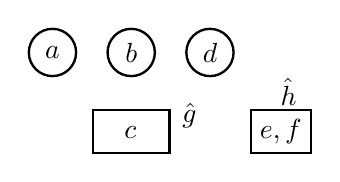
\begin{tikzpicture}
        % Singletons
        \def \ax{0}   \def \ay{0}
        \def \bx{1}   \def \by{0}
        \def \dx{2}   \def \dy{0}
        \def \gx{1}   \def \gy{-1}
        \def \hx{2.9}   \def \hy{-1}

        \draw[line width=0.3mm] (\ax, \ay) circle (0.3) node[anchor=center]{$a$};
        \draw[line width=0.3mm] (\bx, \by) circle (0.3) node[anchor=center]{$b$};
        \draw[line width=0.3mm] (\dx, \dy) circle (0.3) node[anchor=center]{$d$};
        % Cluster

        \node[rectangle, draw, line width=0.3mm] at (\gx, \gy) {$\phantom{a,} c\phantom{, b}$};
        \node at (\gx + 0.74, \gy + 0.2) {$\hat{g}$};

        \node[rectangle, draw, line width=0.3mm] at (\hx, \hy) {$e,f$};
        \node at (\hx + 0.1, \hy + 0.5) {$\hat{h}$};

        % Attacks
        \DrawAttackDiagonal{NRL}{\hx}{\hy+0.1}{\dx}{\dy}
        \DrawAttackVertical{D}{\bx}{\by}{\gx}{\gy}
        \DrawAttackDiagonal{NRL}{\gx-0.1}{\gy+0.1}{\ax}{\ay}
    \end{tikzpicture}
    \caption{Concretized AF $\hat{F}'$ after Step 3}
    \label{example:algorithmConcretizeSingletonsStep3}
\end{figure}
\vspace{-0.2cm}

\begin{algorithm}[H]
    \caption{Concretizing Singletons Pseudocode Step 3}\label{alg:concretizingSingletonsStep3}
    \begin{algorithmic}[1]
        \Require $A: AF(a_1, r_1)$ \Comment{Abstract Clustered AF}
        \Require $C: AF(a_2, r_2)$ \Comment{Concrete AF}
        \Require $N: AF(a_3, r_3)$ \Comment{Concretized Cluster}
        \For{$r_i$ in $A_{r_1}$}
            \If{$r_i.defender$ is cluster and $r_i.attacker$ is cluster}
                \If{!($r_i.attacker$ attacks any of $C[r_i].defender$)}
                    \State $N.removeAttack(r_i)$
                    \State continue
                \EndIf
            \EndIf
            \If{$r_i.defender$ is cluster}
                \If{!($r_i.attacker$ attacks any of $C[r_i].defender$)}
                    \State $N.removeAttack(r_i)$
                    \State continue
                \EndIf
            \EndIf
            \If{$r_i.attacker$ is cluster}
                \If{!($r_i.defender$ defends against any $C[r_i].attacker$)}
                    \State $N.removeAttack(r_i)$
                    \State continue
                \EndIf
            \EndIf
        \EndFor
    \end{algorithmic}
\end{algorithm}


\paragraph{Step 4:} In this step we add the new attacks between the singletons. Due to the fact, that we copied all the attacks from $\hat{F}$, we only have to take into consideration the attacks from or to the concretized singletons. So instead of iterating over all singletons of the AF $\hat{F}'$, we can limit the attack creation to the concretized singletons. The resulting AF is depicted in \cref{example:algorithmConcretizeSingletonsStep4} and the pseudo-code in \cref{alg:concretizingSingletonsStep4}.


\vspace{0.3cm}
\begin{figure}[h]
    \centering
    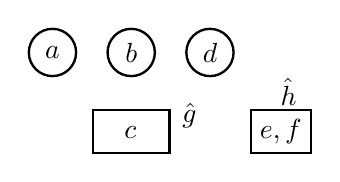
\begin{tikzpicture}
        % Singletons
        \def \ax{0}   \def \ay{0}
        \def \bx{1}   \def \by{0}
        \def \dx{2}   \def \dy{0}
        \def \gx{1}   \def \gy{-1}
        \def \hx{2.9}   \def \hy{-1}

        \draw[line width=0.3mm] (\ax, \ay) circle (0.3) node[anchor=center]{$a$};
        \draw[line width=0.3mm] (\bx, \by) circle (0.3) node[anchor=center]{$b$};
        \draw[line width=0.3mm] (\dx, \dy) circle (0.3) node[anchor=center]{$d$};
        % Cluster

        \node[rectangle, draw, line width=0.3mm] at (\gx, \gy) {$\phantom{a,} c\phantom{, b}$};
        \node at (\gx + 0.74, \gy + 0.2) {$\hat{g}$};

        \node[rectangle, draw, line width=0.3mm] at (\hx, \hy) {$e,f$};
        \node at (\hx + 0.1, \hy + 0.5) {$\hat{h}$};

        % Attacks
        \DrawAttackDiagonal{NRL}{\hx}{\hy+0.1}{\dx}{\dy}
        \DrawAttackVertical{D}{\bx}{\by}{\gx}{\gy}
        \DrawAttackDiagonal{NRL}{\gx-0.1}{\gy+0.1}{\ax}{\ay}
        \DrawAttackHorizontal{L}{\dx}{\dy}{\bx}{\by}
        \DrawAttackHorizontal{L}{\bx}{\by}{\ax}{\ay}
    \end{tikzpicture}
    \caption{Concretized AF $\hat{F}'$ after Step 4}
    \label{example:algorithmConcretizeSingletonsStep4}
\end{figure}
\vspace{-0.2cm}


\begin{algorithm}[H]
    \caption{Concretizing Singletons Pseudocode Step 4}\label{alg:concretizingSingletonsStep4}
    \begin{algorithmic}[1]
        \Require $A: AF(a_1, r_1)$ \Comment{Abstract Clustered AF}
        \Require $C: AF(a_2, r_2)$ \Comment{Concrete AF}
        \Require $e: list(Arguments)$ \Comment{Concretizer List}
        \Require $N: AF(a_3, r_3)$ \Comment{Concretized Cluster}
        \For{$e_i$ in $e$}
            \For{$a_i$ in $C[e_i].attacks$}
                \If{$a_i$ is singleton and ($e_i$, $a_i$) not in $r_2$}
                    \State $N.addAttack((e_i, a_i))$
                \EndIf
            \EndFor
            \For{$a_i$ in $C[e_i].defends$}
                \If{$a_i$ is singleton and ($a_i$, $e_i$) not in $r_2$}
                    \State $N.addAttack((a_i, e_i))$
                \EndIf
            \EndFor
        \EndFor
    \end{algorithmic}
\end{algorithm}


\paragraph{Step 5:} The last step is to clean up the argumentation framework $\hat{F}'$ by removing all empty clusters and mutating the clusters with exactly
one singleton to the mentioned singleton. The resulting AF $\hat{F}'$ is depicted in \cref{example:algorithmConcretizeSingletonsStep5} and the pseudo-code in \cref{alg:concretizingSingletonsStep5}.


\vspace{0.3cm}
\begin{figure}[h!]
    \centering
    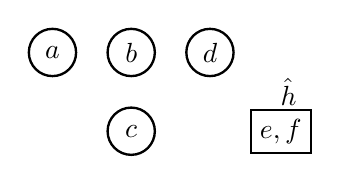
\begin{tikzpicture}
        % Singletons
        \def \ax{0}   \def \ay{0}
        \def \bx{1}   \def \by{0}
        \def \dx{2}   \def \dy{0}
        \def \cx{1}   \def \cy{-1}
        \def \hx{2.9}   \def \hy{-1}

        \draw[line width=0.3mm] (\ax, \ay) circle (0.3) node[anchor=center]{$a$};
        \draw[line width=0.3mm] (\bx, \by) circle (0.3) node[anchor=center]{$b$};
        \draw[line width=0.3mm] (\cx, \cy) circle (0.3) node[anchor=center]{$c$};
        \draw[line width=0.3mm] (\dx, \dy) circle (0.3) node[anchor=center]{$d$};
        % Cluster
        \node[rectangle, draw, line width=0.3mm] at (\hx, \hy) {$e,f$};
        \node at (\hx + 0.1, \hy + 0.5) {$\hat{h}$};

        % Attacks
        \DrawAttackDiagonal{NRL}{\hx}{\hy+0.1}{\dx}{\dy}
        \DrawAttackVertical{D}{\bx}{\by}{\cx}{\cy}
        \DrawAttackDiagonal{NRL}{\cx}{\cy}{\ax}{\ay}
        \DrawAttackHorizontal{L}{\dx}{\dy}{\bx}{\by}
        \DrawAttackHorizontal{L}{\bx}{\by}{\ax}{\ay}
    \end{tikzpicture}
    \caption{Concretized AF $\hat{F}'$ after Step 5}
    \label{example:algorithmConcretizeSingletonsStep5}
\end{figure}
\vspace{-0.2cm}

\begin{algorithm}[H]
    \caption{Concretizing Singletons Pseudocode Step 5}\label{alg:concretizingSingletonsStep5}
    \begin{algorithmic}[1]
        \Require $A: AF(a_1, r_1)$ \Comment{Abstract Clustered AF}
        \Require $C: AF(a_2, r_2)$ \Comment{Concrete AF}
        \Require $e: list(Arguments)$ \Comment{Concretizer List}
        \Require $N: AF(a_3, r_3)$ \Comment{Concretized Cluster}
        \For{$c_i$ in $N.clusters$}
            \If{$c_i.argAmount == 1$}
                \State $c_i \gets Singleton$
            \ElsIf{$c_i.argAmount == 0$}
                \State $N.remove(c_i)$
            \EndIf
        \EndFor
    \end{algorithmic}
\end{algorithm}


\newpage
\section{Computation of Concretizer List}
\label{sec:ComputationOfConcretizerList}
% Why do we need the algorithm
When talking about clustering AFs, faithfulness is an important property. If an AF is spurious, we found atleast one semantics extension, which cannot be mapped to a concrete extension. Based on the spurious extensions, we try to mutate the clustered AF, to obtain faithfulness. This mutation is realized through the concretizer list.

% What is concretizer list
The concretizer list is a list of sets of clustered arguments. Each set is a unique combination of arguments, which are being concretized to find a faithful AF. All the sets of the concretizer list are attempted iteratively, where the order is dependend on the size of the set. We use a heuristicical approach, putting the main focus on local changes. Here we operate directly on the arguments and its attackers which make a set spurious, instead of applying global changes to the AF. Further, a minimal deviation of the abstract AF is usually desired, so small concretizer sets are checked first.

% Input: spurious set
The input to the computation of the concretizer list is a set of the arguments of all the spurious semantics extensions. The size and computation intensity of the concretizer list is highly dependent on the amount of attacks, each argument of the input set and its neighbours with depth 2 have. This is also the critical part of the faithful AF computation and makes some AFs infeasible to solve.

% Example base
Let us have a look at an example to demonstrate how the concretizer list is computed. The concrete AF $G$ is defined in \cref{af:algorithmConcretizer1} and the according abstract AF $\hat{G}$ in \cref{af:algorithmConcretizer2}.


\vspace{0.3cm}
\begin{figure}[h]
\begin{minipage}{.5\textwidth}
    \centering
    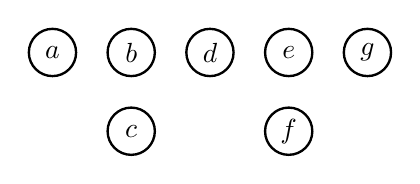
\begin{tikzpicture}
        % Singletons
        \def \ax{0}   \def \ay{0}
        \def \bx{1}   \def \by{0}
        \def \cx{1}   \def \cy{-1}
        \def \dx{2}   \def \dy{0}
        \def \ex{3}   \def \ey{0}
        \def \fx{3}   \def \fy{-1}
        \def \gx{4}   \def \gy{0}

        \draw[line width=0.3mm] (\ax, \ay) circle (0.3) node[anchor=center]{$a$};
        \draw[line width=0.3mm] (\bx, \by) circle (0.3) node[anchor=center]{$b$};
        \draw[line width=0.3mm] (\cx, \cy) circle (0.3) node[anchor=center]{$c$};
        \draw[line width=0.3mm] (\dx, \dy) circle (0.3) node[anchor=center]{$d$};
        \draw[line width=0.3mm] (\ex, \ey) circle (0.3) node[anchor=center]{$e$};
        \draw[line width=0.3mm] (\fx, \fy) circle (0.3) node[anchor=center]{$f$};
        \draw[line width=0.3mm] (\gx, \gy) circle (0.3) node[anchor=center]{$g$};

        % Attacks
        \DrawSelfAttackLeftSingleton{\ax}{\ay}
        \DrawAttackHorizontal{B}{\bx}{\by}{\ax}{\ay}
        \DrawAttackHorizontal{R}{\bx}{\by}{\dx}{\dy}
        \DrawAttackHorizontal{B}{\ex}{\ey}{\dx}{\dy}
        \DrawAttackHorizontal{R}{\ex}{\ey}{\gx}{\gy}
        \DrawAttackVertical{B}{\bx}{\by}{\cx}{\cy}
        \DrawAttackVertical{D}{\ex}{\ey}{\fx}{\fy}
        \DrawAttackDiagonal{PLR}{\fx}{\fy}{\gx}{\gy}
    \end{tikzpicture}
    \subcaption{Concrete AF $G$}
    \label{af:algorithmConcretizer1}
\end{minipage}%
\begin{minipage}{.5\textwidth}
    \centering
    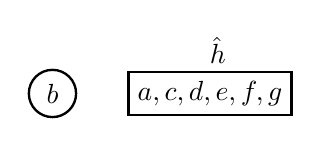
\begin{tikzpicture}
        % Singletons
        \def \bx{0}   \def \by{0}
        \def \hx{2}   \def \hy{0}

        \draw[line width=0.3mm] (\bx, \by) circle (0.3) node[anchor=center]{$b$};

        % Cluster
        \node[rectangle, draw, line width=0.3mm] at (\hx, \hy) {$a, c, d, e, f, g$};
        \node at (\hx + 0.1, \hy + 0.55) {$\hat{h}$};
        % Attacks
        \DrawAttackHorizontal{B}{\hx-0.85}{\hy}{\bx}{\by}
        \DrawSelfAttackRightTopCluster{\hx+1}{\hy+0.29}

    \end{tikzpicture}
    \subcaption{Abstract AF $\hat{G}$}
    \label{af:algorithmConcretizer2}
\end{minipage}
\caption{Concrete and abstract AF}
\label{fig:comparison}
\end{figure}
\vspace{0.3cm}

If we have a look at the stable extensions of the concrete AF $G$, e.g.\ 
$\mathtt{stb=}\bigl\{\{b, c\}\bigl\}$ and at the abstractly stable extensions of the abstract AF $\hat{G}$, e.g.\ 
$\mathtt{\hat{stb}=}\bigl\{\{b, \hat{h}\}, \{\hat{h}\}, \{b\}\bigl\}$, we can see that the abstractly stable extensions $\{\hat{h}\}$ and $\{b\}$ are spurious. The input to the concretizer list computation is a collection of the arguments of all the spurious sets, which in this case is $\{b, \hat{h}\}$.

% Filter Cluster out of spurious set, because we cant concretize cluster
The first step is to filter out the clusters of the input, since clusters are not present in the concrete AF and therefore do not attack any singletons and are not being attacked. So we reduce the concretizer list from $\{b, \hat{h}\}$ to $\{b\}$. The pseudo-code is listed in \cref{alg:concretizerListPrefiltering}.

\begin{algorithm}[H]
    \caption{Computation of Concretizer list Algorithm: Prefiltering}\label{alg:concretizerListPrefiltering}
    \begin{algorithmic}[1]
        \Require $\hat{G}: AF(a_2, r_2)$ \Comment{Abstract AF}
        \Require $s: list(Arguments)$ \Comment{spurious arguments}
        \For{$s_i$ in $s$}
            \If{$s_i$ in $\hat{G}$ is cluster}
                \State $s$.remove($s_i$)
            \EndIf
        \EndFor
    \end{algorithmic}
\end{algorithm}

% Get combination as attacker depth 2
% Get combination as defender depth 2
Next, we have a look at the neighbouring arguments of the current concretizer list.  Neighbours in this context are arguments which attack, or are being attacked by an argument. The depth defines how many arguments are between the attacks. A depth of $0$ is the actual argument, a depth of $1$ represents the direct attacker of the argument and the direct arguments, which are being attacked by the argument. A depth $2$ argument is an argument, which has some attack relation (e.g.\ attacks the argument or is attacked by the argument) with a depth $1$ argument.

We used a search depth of $2$ in our implementation. So when having a look at our example, we take the defender of depth $1$ and $2$, in \cref{af:algorithmConcretizer3} depicted in yellow and the attacker with the same depth, depicted in blue. The pseudo-code of this procedure is listed in \cref{alg:concretizerListNeighbours}. Some arguments can have multiple depths (e.g.\ argument $c$. It is a direct attacker of the argument $b$ with depth $0$, but also a direct attacker of the argument $c$ with depth $1$), than the lower depth is chosen as the representative.

%Depth 2 Attacker
\vspace{0.1cm}
\begin{figure}[h!]
    \centering
    \begin{tikzpicture}
        % Singletons
        \def \ax{0}   \def \ay{0}
        \def \bx{1}   \def \by{0}
        \def \cx{1}   \def \cy{-1}
        \def \dx{2}   \def \dy{0}
        \def \ex{3}   \def \ey{0}
        \def \fx{3}   \def \fy{-1}
        \def \gx{4}   \def \gy{0}

        \draw[line width=0.3mm] (\ax, \ay) circle (0.3) node[anchor=center]{$a$};
        \draw[cYellow] (\ax,\ay) circle (0.4);
        \node[text=cYellow] at (\ax+0.33, \ay+0.45) {\footnotesize 1};

        \draw[line width=0.3mm] (\bx, \by) circle (0.3) node[anchor=center]{$b$};
        \draw[cRed] (\bx,\by) circle (0.4);
        \node[text=cRed] at (\bx+0.33, \by+0.45) {\footnotesize 0};

        \draw[line width=0.3mm] (\cx, \cy) circle (0.3) node[anchor=center]{$c$};
        \draw[cYellow] (\cx,\cy) circle (0.4);
        \node[text=cYellow] at (\cx+0.55, \cy) {\footnotesize 1};

        \draw[line width=0.3mm] (\dx, \dy) circle (0.3) node[anchor=center]{$d$};
        \draw[cBlue] (\dx,\dy) circle (0.4);
        \node[text=cBlue] at (\dx+0.33, \dy+0.45) {\footnotesize 1};

        \draw[line width=0.3mm] (\ex, \ey) circle (0.3) node[anchor=center]{$e$};
        \draw[cBlue] (\ex,\ey) circle (0.4);
        \node[text=cBlue] at (\ex+0.33, \ey+0.45) {\footnotesize 2};

        \draw[line width=0.3mm] (\fx, \fy) circle (0.3) node[anchor=center]{$f$};
        \node at (\fx+0.45, \fy) {\footnotesize 3};

        \draw[line width=0.3mm] (\gx, \gy) circle (0.3) node[anchor=center]{$g$};
        \node at (\gx+0.33, \gy+0.45) {\footnotesize 3};

        % Attacks
        \DrawSelfAttackLeftSingleton{\ax}{\ay}
        \DrawSelfAttackLeftSingleton{\cx}{\cy}
        \DrawAttackHorizontal{B}{\bx}{\by}{\ax}{\ay}
        \DrawAttackHorizontal{R}{\bx}{\by}{\dx}{\dy}
        \DrawAttackHorizontal{B}{\ex}{\ey}{\dx}{\dy}
        \DrawAttackHorizontal{R}{\ex}{\ey}{\gx}{\gy}
        \DrawAttackVertical{B}{\bx}{\by}{\cx}{\cy}
        \DrawAttackVertical{D}{\ex}{\ey}{\fx}{\fy}
        \DrawAttackDiagonal{PLR}{\fx}{\fy}{\gx}{\gy}
    \end{tikzpicture}
    \caption{Singletons depth with $b$ as viewpoint}
    \label{af:algorithmConcretizer3}
\end{figure}
\vspace{-0.2cm}

\begin{algorithm}
    \caption{Computation of Concretizer list Algorithm: Neighbours}\label{alg:concretizerListNeighbours}
    \begin{algorithmic}[1]
        \Require $G: AF(a_1, r_1)$ \Comment{Concrete AF}
        \Require $s: list(Arguments)$ \Comment{Working List}
        \State $N$ $\gets$ $[]$ \Comment{$N$ = list of neighbours}
        \For{$s_i$ in $s$} \Comment{Get neighbours}
            \For{$n(1)_i$ neighbour of $s_i$} \Comment{depth 1 attacker}
                \For{$n(2)_i$ neighbour of $n(1)_i$} \Comment{depth 2 attacker}
                    \State $N.append(n(1)_i$)
                    \State $N.append(n(2)_i$)
                \EndFor
            \EndFor
        \EndFor
    \end{algorithmic}
\end{algorithm}


Now the concretizer list is expanded with all the possible combinations of the neighbours. The neighbours of the current example are $\{a, c, d, e\}$. When building the combinations, we create the table defined in \cref{table:algorithmConcretizer1}.

\begin{table}[htb]
    \centering
    \begin{tabular}{ |c|c|c|c| }
     \hline
     size $1$ & size $2$ & size $3$ & size $4$\\
     \hline
     \hline
     $\{a\}$ & $\{a, c\}$ & $\{a, c, d\}$ &$\{a, c, d, e\}$ \\
     \hline
     $\{c\}$ & $\{a, d\}$ & $\{a, c, e\}$ & \\
     \hline
     $\{d\}$ & $\{a, e\}$ & $\{a, d, e\}$ & \\
     \hline
     $\{e\}$ & $\{c, d\}$ & $\{c, d, e\}$ & \\
     \hline
       & $\{c, e\}$ &  & \\
     \hline
       & $\{d, e\}$ &  & \\
     \hline
    \end{tabular}
\caption{Combinations of $\{a, c, d, e\}$}
\label{table:algorithmConcretizer1}

\end{table}

The combination table grows exponentially to the base of 2. Therefore, the size of the neighbours is crucial. If we have too many neighbours, the computation would need too much memory and turns infeasible to compute.

% Add concretizer list defined by the user
% deduplicate
If the user has provided arguments which have to be concretized as program argument, we add them to each combination set. After adding them, we filter for duplicates to keep the concretizer list size to a minimum.

% Filter singletons which are not in cluster, because cant concretize singletons
% deduplicate
Next, we need to filter out the arguments, which are not in clusters, since singletons are already concrete. This filtering could lead to some duplicates again, which we need to remove once again to minimize the memory consumption and reduce the amount of faitfhul checks.

Finally, we sort the list by the set size and return it. In the current example we would return the whole table, because no concretizer arguments were provided by the user. So the concretizer list would be
$\bigl\{\{a\}$
$\{b\}$
$\{c\}$
$\{d\}$
$\{a, c\}$
$\{a, d\}$
$\{a, e\}$
$\{c, d\}$
$\{c, e\}$
$\{d, e\}$
$\{a, c, d\}$
$\{a, c, e\}$
$\{a, d, e\}$
$\{c, d, e\}$
$\{a, c, d, e\}\bigl\}$. The pseudo-code for the last step is stated in \cref{alg:concretizerListCombinationAndCleanup}.


\begin{algorithm}
    \caption{Computation of Concretizer list Algorithm: Combinations and Cleanup}\label{alg:concretizerListCombinationAndCleanup}
    \begin{algorithmic}[1]
        \Require $G: AF(a_1, r_1)$ \Comment{Concrete AF}
        \Require $\hat{G}: AF(a_2, r_2)$ \Comment{Abstract AF}
        \Require $s: list(Arguments)$ \Comment{Working List}
        \Require $ca: list(Arguments)$ \Comment{Concretize arguments parameter}

        \State $C \gets$ combinations of N with $range(1, len(N)-1)$ \Comment{Combination List}

        \For{$ca_i$ in $ca$} \Comment{Parameter Arguments to be concretized}
            \For{$c_i$ in $C$}
                \State $c_i.append(ca_i)$
            \EndFor
        \EndFor
        \State $C.deduplicate()$

        \For{$s_i$ in $C$} \Comment{Remove clusters}
            \For{$a_i$ in $s_i$}
                \If{$\hat{G}[a_i]$ is cluster}
                    \State $s_i.remove(a_i)$
                \EndIf
            \EndFor
        \EndFor
        \State \Return $s.sortBySize()$
    \end{algorithmic}
\end{algorithm}

When concretizing the list, we find a set which leads to a faithful AF: $\{a, c, d\}$ depicted in \cref{af:algorithmConcretizer4}.

\begin{figure}[H]
    \centering
    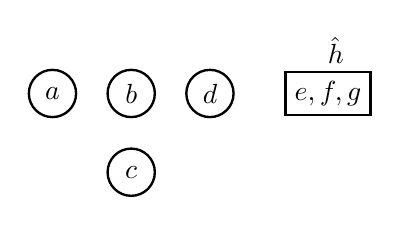
\begin{tikzpicture}
        % Singletons
        \def \ax{0}   \def \ay{0}
        \def \bx{1}   \def \by{0}
        \def \cx{1}   \def \cy{-1}
        \def \dx{2}   \def \dy{0}
        \def \hx{3.5}   \def \hy{0}

        \draw[line width=0.3mm] (\ax, \ay) circle (0.3) node[anchor=center]{$a$};
        \draw[line width=0.3mm] (\bx, \by) circle (0.3) node[anchor=center]{$b$};
        \draw[line width=0.3mm] (\cx, \cy) circle (0.3) node[anchor=center]{$c$};
        \draw[line width=0.3mm] (\dx, \dy) circle (0.3) node[anchor=center]{$d$};

        % Cluster
        \node[rectangle, draw, line width=0.3mm] at (\hx, \hy) {$e, f, g$};
        \node at (\hx + 0.1, \hy + 0.55) {$\hat{h}$};
        % Attacks
        \DrawAttackHorizontal{B}{\hx-0.3}{\hy}{\dx}{\dy}
        \DrawAttackHorizontal{B}{\bx}{\by}{\ax}{\ay}
        \DrawAttackHorizontal{R}{\bx}{\by}{\dx}{\dy}
        \DrawAttackVertical{B}{\bx}{\by}{\cx}{\cy}
        \DrawSelfAttackRightTopCluster{\hx+0.45}{\hy+0.29}
        \DrawSelfAttackLeftSingleton{\ax}{\ay}

    \end{tikzpicture}
    \caption{Faithful AF $\hat{G}'$}
    \label{af:algorithmConcretizer4}
\end{figure}



\newpage

\section{Encodings}
\label{sec:Encodings}
We previously defined the semantics in mathematical notation. But since we use SAT-Solving to obtain semantics sets, we have to bring them into a Boolean form. We will accompany each Boolean formula with an example AF with the according Boolean resolution.


\paragraph{Conflict-Free} A set of arguments is (abstractly) conflict-free, if each argument of the set is \emph{true} and the formula defined in \cref{def:booleanFormulaConflictFree} is satisfiable.

\begin{definition}
    Let $G=(A,R)$ be an AF. Then all the satisfiable of the following formula are (abstract) conflict-free sets.
    \begin{center}
        \[
        \bigwedge_{a \in A_{\!S\!I\!N\!G\!L\!E}} \bigl( \bigwedge_{b:(b,a)\in R, b \in A_{\!S\!I\!N\!G\!L\!E}} \lnot \bigl( a \wedge b \bigl) \bigl)
        \]
    \end{center}
    \label{def:booleanFormulaConflictFree}
\end{definition}


\begin{example}
    Let us have a look at an example and define the AF $G=(A,R)$ to be the AF depicted in \cref{af:algorithmEncodingsConflictFree}. Where the arguments are $A=\{a, b, c, d\}$ and the attacks $R=\big\{ (a,a), (a,b), (b,c), (d,a), (d,b), (d,c)\big\}$.

    \begin{figure}[H]
        \centering
        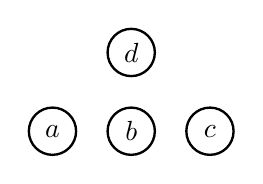
\begin{tikzpicture}
            % Singletons
            \def \ax{0}   \def \ay{-1}
            \def \bx{1}   \def \by{-1}
            \def \cx{2}   \def \cy{-1}
            \def \dx{1}   \def \dy{0}

            \draw[line width=0.3mm] (\ax, \ay) circle (0.3) node[anchor=center]{$a$};
            \draw[line width=0.3mm] (\bx, \by) circle (0.3) node[anchor=center]{$b$};
            \draw[line width=0.3mm] (\cx, \cy) circle (0.3) node[anchor=center]{$c$};
            \draw[line width=0.3mm] (\dx, \dy) circle (0.3) node[anchor=center]{$d$};

            % Attacks
            \DrawAttackHorizontal{R}{\ax}{\ay}{\bx}{\by}
            \DrawAttackHorizontal{R}{\bx}{\by}{\cx}{\cy}
            \DrawSelfAttackLeftSingleton{\ax}{\ay}
            \DrawAttackDiagonal{PRL}{\dx}{\dy}{\ax}{\ay}
            \DrawAttackDiagonal{NLR}{\dx}{\dy}{\cx}{\cy}
            \DrawAttackVertical{D}{\dx}{\dy}{\bx}{\by}
        \end{tikzpicture}
        \caption{Concrete AF $G$}
        \label{af:algorithmEncodingsConflictFree}
    \end{figure}

By applying the conflict-free formula to the AF $G$, we obtain a Boolean expression. For conflict-free, the expression is always satisfiable with the empty set. Every other model that satisfies the formula is also part of the conflict-free set.
\begin{align*}
    \psi =
    \lnot(b \land a)  \land
    \lnot(b \land d)  \land
    & \lnot(a \land d)  \land
    \lnot(a \land a)  \land
    \\
    & \lnot(c \land b)  \land
    \lnot(c \land d)
\end{align*}

The satisfiable models of $\psi$, and thus, the conflict-free sets of the AF $G$ are $\bigl\{$ $\{\}$ $\{b\}$, $\{c\}$, $\{d\}$ $\bigl\}$.
\end{example}


\paragraph{Admissible} Every satisfiable model of \cref{def:booleanFormulaAdmissible} is an (abstractly) admissible set.

\begin{definition}
    Let $G=(A,R)$ be an AF. Then all the satisfiable of the following formula are (abstract) admissible sets.
    \begin{center}
        \[ \bigwedge_{a \in A_{\!S\!I\!N\!G\!L\!E}} \big( \bigwedge_{b:(b,a)\in R, b \in A_{\!S\!I\!N\!G\!L\!E}} \lnot \big( a \wedge b \big)\big) \land  \bigwedge_{a \in A_{\!S\!I\!N\!G\!L\!E}} \big( a \rightarrow \bigwedge_{b:(b,a) \in R} \big( \bigvee_{c:(c,b) \in R} c\big) \big)
        \]
    \end{center}
    \label{def:booleanFormulaAdmissible}
\end{definition}


\begin{example}
    Let us have a look at an example and define the AF $G=(A,R)$ to be the AF depicted in \cref{af:algorithmEncodingsAdmissible}. Where the arguments are $A=\{a, b, c, d, e\}$ and the attacks $R=\big\{ (a,a), (a,b), (b,c), (d,a), (d,b), (d,d), (d, e), (e, d)\big\}$.

    \begin{figure}[H]
        \centering
        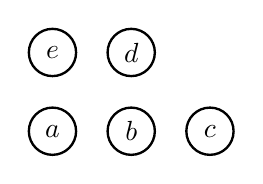
\begin{tikzpicture}
            % Singletons
            \def \ax{0}   \def \ay{-1}
            \def \bx{1}   \def \by{-1}
            \def \cx{2}   \def \cy{-1}
            \def \dx{1}   \def \dy{0}
            \def \ex{0}   \def \ey{0}

            \draw[line width=0.3mm] (\ax, \ay) circle (0.3) node[anchor=center]{$a$};
            \draw[line width=0.3mm] (\bx, \by) circle (0.3) node[anchor=center]{$b$};
            \draw[line width=0.3mm] (\cx, \cy) circle (0.3) node[anchor=center]{$c$};
            \draw[line width=0.3mm] (\dx, \dy) circle (0.3) node[anchor=center]{$d$};
            \draw[line width=0.3mm] (\ex, \ey) circle (0.3) node[anchor=center]{$e$};

            % Attacks
            \DrawAttackHorizontal{R}{\ax}{\ay}{\bx}{\by}
            \DrawAttackHorizontal{R}{\bx}{\by}{\cx}{\cy}
            \DrawAttackHorizontal{B}{\dx}{\dy}{\ex}{\ey}
            \DrawSelfAttackLeftSingleton{\ax}{\ay}
            \DrawSelfAttackRightSingleton{\dx}{\dy}
            \DrawAttackDiagonal{PRL}{\dx}{\dy}{\ax}{\ay}
            \DrawAttackVertical{D}{\dx}{\dy}{\bx}{\by}
        \end{tikzpicture}
        \caption{Concrete AF $G$}
        \label{af:algorithmEncodingsAdmissible}
    \end{figure}

By applying the admissible formula to the AF $G$, we obtain a Boolean expression. For admissible, the empty set does always satisfy the formula and therefore is always part of the admissible sets. Besides the empty set, every model which satisfies the formula is also part of the admissible sets.
\begin{align*}
    \psi = \big(
    \lnot (a \land a)
    & \land \lnot (a \land d) \land \lnot (b \land d) \land \lnot (b \land c) \land \lnot (b \land d) \land \lnot (c \land b) \land \lnot (d \land e) \\
    & \land \lnot (d \land d) \land \lnot (e \land d) \big) \\
    & \land \bigl( a \rightarrow ((a \lor d) \land (e \lor d)) \land \bigl( b \rightarrow ((a \lor d) \land (b) \land (e \lor d)) \bigl) \bigl)\\
    & \land \bigl( c \rightarrow (a \lor c \lor d) \bigl) \land \bigl( d \rightarrow (d) \land (e \lor d) \bigl) \land \bigl( e \rightarrow (e \lor d) \bigl)
\end{align*}

The satisfiable models of $\psi$, and thus, the admissible sets of the AF $G$ are $\big\{ \{\},$ $\{e\},$ $\{c, e\}$ $\big\}$.
\end{example}



\paragraph{Stable} Every satisfiable model of \cref{def:booleanFormulaStable} is a (abstractly) stable extension.


\begin{definition}
    Let $G=(A,R)$ be an AF. Then all the satisfiable of the following formula are (abstractly) stable extensions.
    \begin{center}
        \[
        \bigwedge_{a \in A_{\!S\!I\!N\!G\!L\!E}} \big( \bigwedge_{b:(b,a)\in R, b \in A_{\!S\!I\!N\!G\!L\!E}} \lnot \big( a \wedge b \big) \big) \land \bigwedge_{a \in A} \big( a \bigvee_{b:(b,a)\in R} b\big) \land \bigwedge_{a \in A} \big( \big(  a \bigwedge_{b:(b,a) \in R} \lnot b\big)  \rightarrow \big( \bigwedge_{c:(a,c), c \in A_{\!S\!I\!N\!G\!L\!E}} \lnot c\big) \big)
        \]
    \end{center}
    \label{def:booleanFormulaStable}
\end{definition}


\begin{example}
    Let us have a look at an example and define the AF $G=(A,R)$ to be the AF depicted in \cref{af:algorithmEncodingsStable}. Where the arguments are $A=\{a, b, c, d\}$ and the attacks $R=\big\{ (a,a), (a,b), (a,d), (b,a), (b,d), (c,b), (d,a)\big\}$.

    \begin{figure}[H]
        \centering
        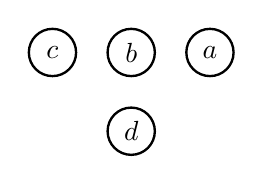
\begin{tikzpicture}
            % Singletons
            \def \ax{2}   \def \ay{0}
            \def \bx{1}   \def \by{0}
            \def \cx{0}   \def \cy{0}
            \def \dx{1}   \def \dy{-1}

            \draw[line width=0.3mm] (\ax, \ay) circle (0.3) node[anchor=center]{$a$};
            \draw[line width=0.3mm] (\bx, \by) circle (0.3) node[anchor=center]{$b$};
            \draw[line width=0.3mm] (\cx, \cy) circle (0.3) node[anchor=center]{$c$};
            \draw[line width=0.3mm] (\dx, \dy) circle (0.3) node[anchor=center]{$d$};

            % Attacks
            \DrawSelfAttackRightSingleton{\ax}{\ay}
            \DrawAttackHorizontal{R}{\cx}{\cy}{\bx}{\by}
            \DrawAttackHorizontal{B}{\ax}{\ay}{\bx}{\by}
            \DrawAttackVertical{D}{\bx}{\by}{\dx}{\dy}
            \DrawAttackDiagonal{PLR}{\dx}{\dy}{\ax}{\ay}
        \end{tikzpicture}
        \caption{Concrete AF $G$}
        \label{af:algorithmEncodingsStable}
    \end{figure}

If we apply the stable extension formula, we obtain the following Boolean expression. In contrast to conflict-free and admissible, the empty set does not satisfy the expression and therefore is not part of the stable extensions.

\begin{align*}
    \psi = \bigl( (\lnot (a \land a)) \land (\lnot (a \land b)) &\land (\lnot (a \land d)) \land (\lnot (b \land a)) \land (\lnot (b \land c)) \land (\lnot (d \land b)) \land (\lnot (d \land a)) \bigl) \\
    &\land \bigl( (a \lor a \lor b \lor d) \land (a \lor b \lor c) \land (a \lor b \lor d) \bigl) \\
    &\land \bigl( ((a \land \lnot a \land \lnot b \land \lnot d) \rightarrow (\lnot a \land \lnot b \land \lnot d)\bigl)\\
    &\land \bigl((b \land \lnot a \land \lnot c) \rightarrow \lnot a \land \lnot d) \land ((d \land \lnot b \land \lnot a) \rightarrow \lnot a)\bigl)
\end{align*}


The satisfiable models of $\psi$, and therefore, the stable extensions of the AF $G$ is $\bigl\{ \{c, d\}\bigl\}$.
\end{example}

\newpage

\section{Algorithmic Approach to Compute Faifthul Clusterings}
\label{sec:AlgorithmicApproachToComputeFaifthulClusterings}
\textit{TODO: Concretize singletons of clustered AF algorithm}

\section{Heuristics and Refinements}
\label{sec:HeuristicsAndRefinements}
\textit{TODO: Define every Heuristic and refinement we used for each semantic}
